%=======================02-713 LaTeX template, following the 15-210 template==================
%
% You don't need to use LaTeX or this template, but you must turn your homework in as
% a typeset PDF somehow.
%
% How to use:
%    1. Update your information in section "A" below
%    2. Write your answers in section "B" below. Precede answers for all 
%       parts of a question with the command "\question{n}{desc}" where n is
%       the question number and "desc" is a short, one-line description of 
%       the problem. There is no need to restate the problem.
%    3. If a question has multiple parts, precede the answer to part x with the
%       command "\part{x}".
%    4. If a problem asks you to design an algorithm, use the commands
%       \algorithm, \correctness, \runtime to precede your discussion of the 
%       description of the algorithm, its correctness, and its running time, respectively.
%    5. You can include graphics by using the command \includegraphics{FILENAME}
%
\documentclass[11pt]{article}
\usepackage{amsmath,amssymb,amsthm}
\usepackage{graphicx}
\usepackage[margin=1in]{geometry}
\usepackage{fancyhdr}
\usepackage{listings}
\setlength{\parindent}{0pt}
\setlength{\parskip}{5pt plus 1pt}
\setlength{\headheight}{13.6pt}
\newcommand\question[2]{\vspace{.25in}\hrule\textbf{#1: #2}\vspace{.5em}\hrule\vspace{.10in}}
\renewcommand\part[1]{\vspace{.10in}\textbf{(#1)}}
\newcommand\algorithm{\vspace{.10in}\textbf{Algorithm: }}
\newcommand\ot{\vspace{.10in}\textbf{Output: }}
\newcommand\runtime{\vspace{.10in}\textbf{Running time: }}
\pagestyle{fancyplain}
\lhead{\textbf{\NAME\ (\ANDREWID)}}
\chead{\textbf{Lab\HWNUM}}
\rhead{\today}
\begin{document}\raggedright
%Section A==============Change the values below to match your information==================
\newcommand\NAME{Yao Xiao}  % your name
\newcommand\ANDREWID{2019180015}     % your andrew id
\newcommand\HWNUM{5}              % the homework number
%Section B==============Put your answers to the questions below here=======================

% no need to restate the problem --- the graders know which problem is which,
% but replacing "The First Problem" with a short phrase will help you remember
% which problem this is when you read over your homeworks to study.

\question{1}{The First Problem} 

\part{a} \algorithm
\begin{lstlisting}
import numpy as np

class KMeansClassifier():
    def __init__(self, k=3, initCent='random', max_iter=500):

        self._k = k
        self._initCent = initCent
        self._max_iter = max_iter
        self._clusterAssment = None
        self._labels = None
        self._sse = None

    def _calEDist(self, arrA, arrB):
        return np.math.sqrt(sum(np.power(arrA - arrB, 2)))

    def _calMDist(self, arrA, arrB):
        return sum(np.abs(arrA - arrB))

    def _randCent(self, data_X, k):
        n = data_X.shape[1]
        centroids = np.empty((k, n))
        for j in range(n):
            minJ = min(data_X[:, j])
            rangeJ = float(max(data_X[:, j] - minJ))
            # 使用flatten拉平嵌套列表(nested list)
            centroids[:, j] = (minJ + rangeJ * np.random.rand(k, 1)).flatten()
        return centroids

    def fit(self, data_X):
        if not isinstance(data_X, np.ndarray) or \
                isinstance(data_X, np.matrixlib.defmatrix.matrix):
            try:
                data_X = np.asarray(data_X)
            except:
                raise TypeError("numpy.ndarray resuired for data_X")

        m = data_X.shape[0]
        self._clusterAssment = np.zeros((m, 2))

        if self._initCent == 'random':
            self._centroids = self._randCent(data_X, self._k)

        clusterChanged = True
        for _ in range(self._max_iter):
            clusterChanged = False
            for i in range(m):
                min_dist = np.inf
                min_index = -1
                for j in range(self._k):
                    arrA = self._centroids[j, :]
                    arrB = data_X[i, :]
                    dist = self._calEDist(arrA, arrB)
                    if dist < min_dist:
                        min_dist = dist
                        min_index = j
                if self._clusterAssment[i, 0] != min_index or self._clusterAssment[i, 1] > min_dist ** 2:
                    clusterChanged = True
                    self._clusterAssment[i, :] = min_index, min_dist ** 2
            if not clusterChanged:
                break
            for i in range(self._k):
                index_all = self._clusterAssment[:, 0]
                value = np.nonzero(index_all == i)
                ptsInClust = data_X[value[0]]
                self._centroids[i, :] = np.mean(ptsInClust, axis=0)

        self._labels = self._clusterAssment[:, 0]
        self._sse = sum(self._clusterAssment[:, 1])

    def predict(self, X):
        if not isinstance(X, np.ndarray):
            try:
                X = np.asarray(X)
            except:
                raise TypeError("numpy.ndarray required for X")

        m = X.shape[0]
        preds = np.empty((m,))
        for i in range(m):
            min_dist = np.inf
            for j in range(self._k):
                dist = self._calEDist(self._centroids[j, :], X[i, :])
                if dist < min_dist:
                    min_dist = dist
                    preds[i] = j
        return preds

    @property
    def sse(self):
        return self._sse

    @property
    def labels(self):
        return self._labels

    @property
    def centroids(self):
        return self._centroids

\end{lstlisting}

\question{2}{The second problem}

\part{a} \algorithm
\begin{lstlisting}
import pandas as pd
import numpy as np
from lab5 import KMeansClassifier
import matplotlib.pyplot as plt
from sklearn import datasets

if __name__ == '__main__':
    iris = datasets.load_iris()
    X = iris.data
    data_X = X[:, [1, 3]]
    k = 3
    clf = KMeansClassifier(k)
    clf.fit(data_X)
    cents = clf.centroids
    labels = clf.labels
    sse = clf.sse
    colors = ['b', 'g', 'r', 'k', 'c', 'm', 'y', '#e24fff', '#524C90', '#845868']
    for i in range(k):
        index = np.nonzero(labels == i)[0]
        x0 = data_X[index, 0]
        x1 = data_X[index, 1]
        y_i = i
        for j in range(len(x0)):
            plt.text(x0[j], x1[j], str(y_i), color=colors[i], \
                     fontdict={'weight': 'bold', 'size': 6})
        plt.scatter(cents[i, 0], cents[i, 1], marker='x', color=colors[i], \
                    linewidths=7)

    plt.title("k=" + str(k) + "  SSE={:.2f}".format(sse))
    plt.axis([-7, 7, -7, 7])
    output = str(k) + ".png"
    plt.savefig(output)
    plt.show()
    
\end{lstlisting}


\part{b} \ot
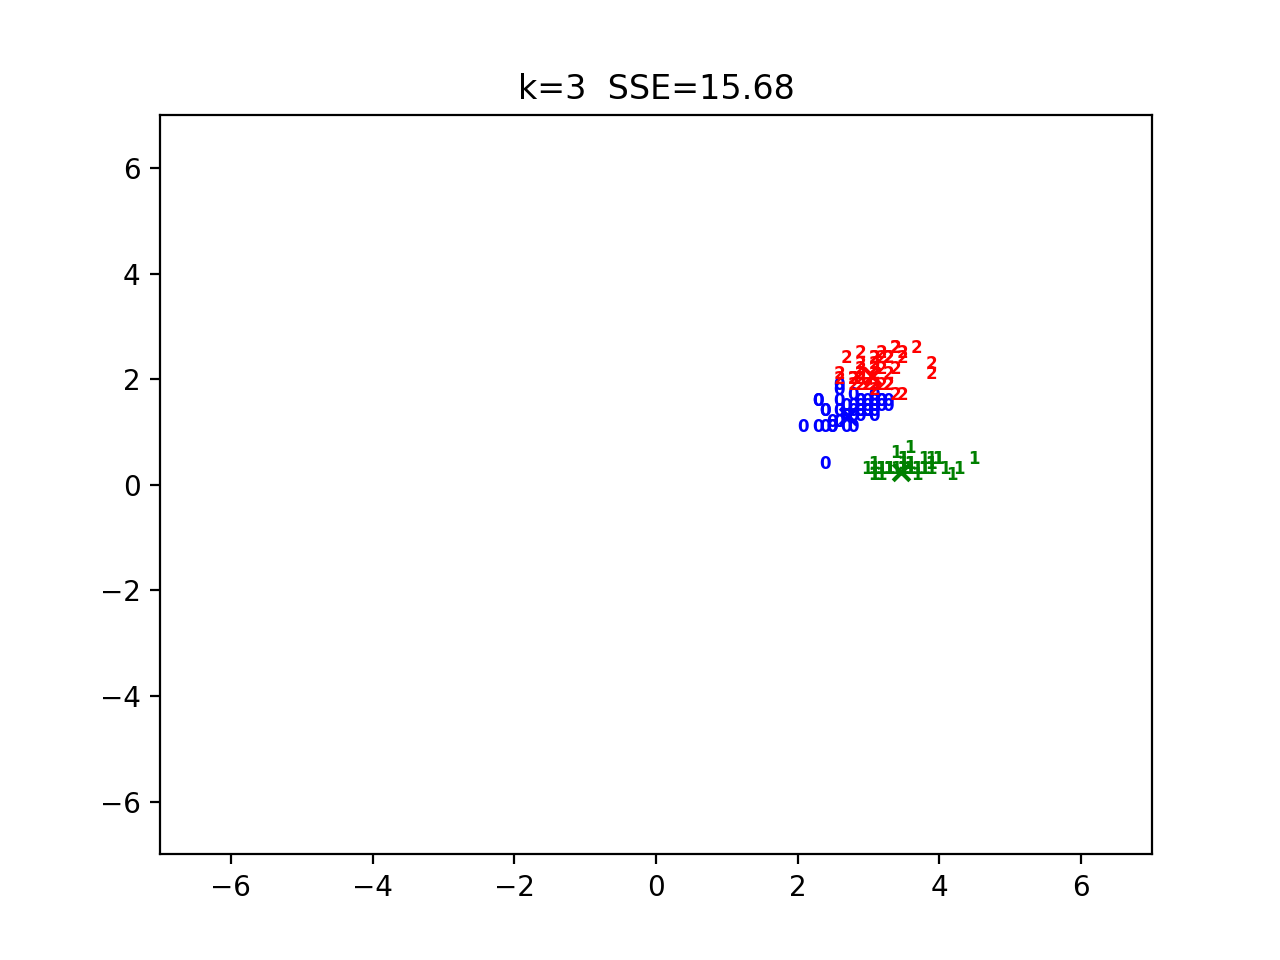
\includegraphics{Figure_1.png}
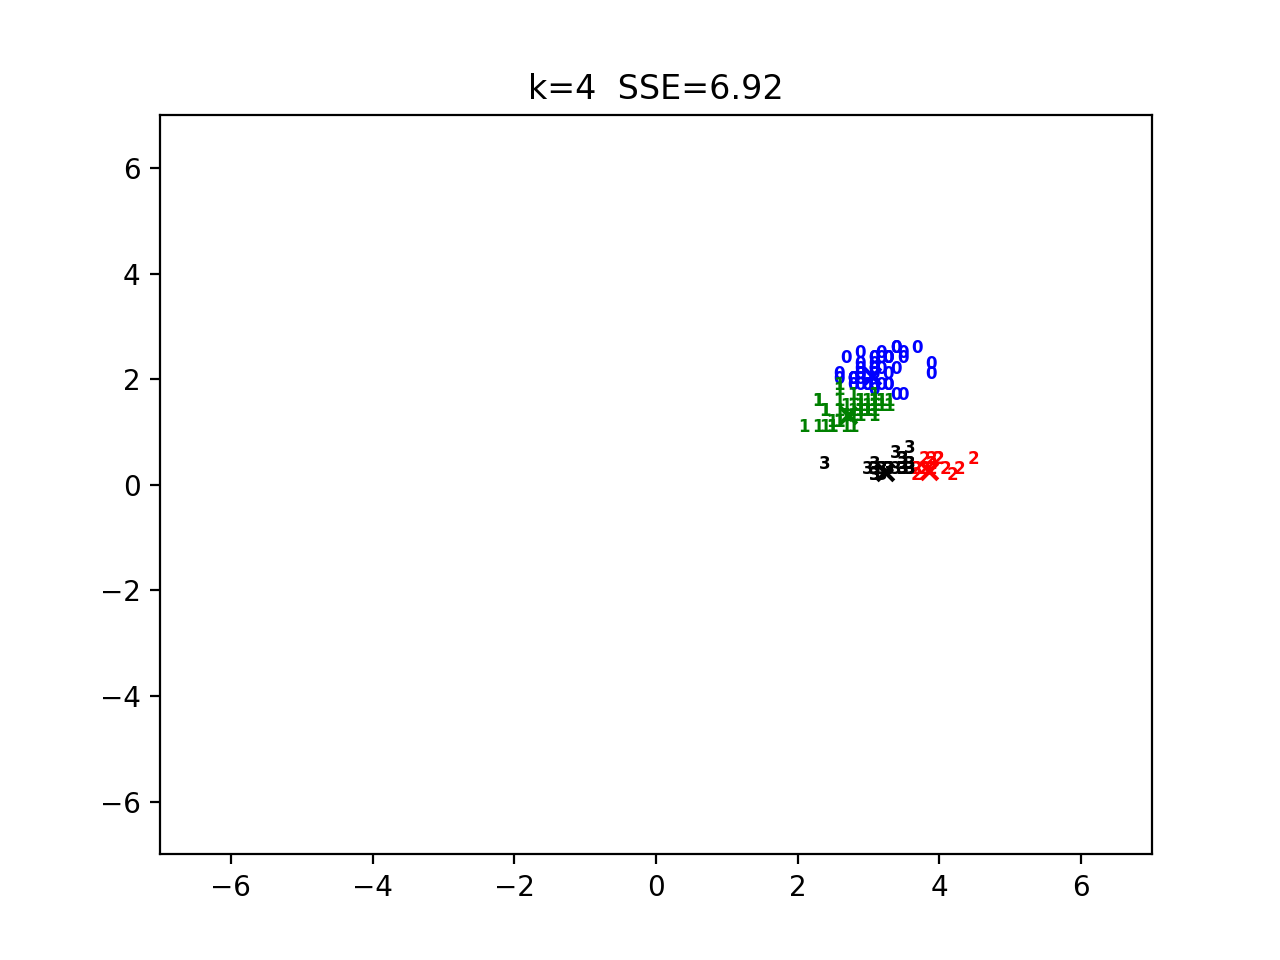
\includegraphics{Figure_2.png}
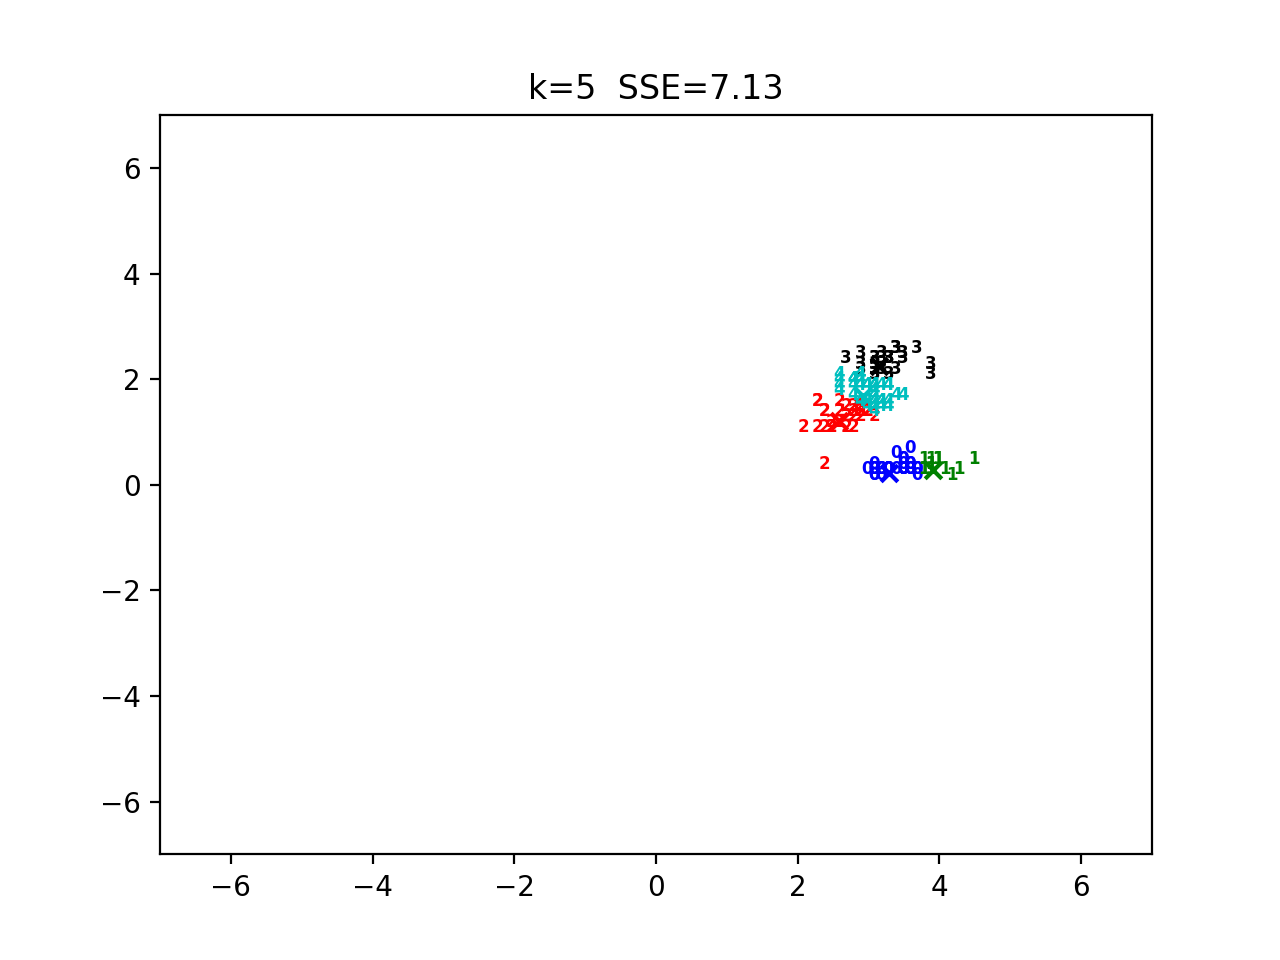
\includegraphics{Figure_3.png}

\end{document}
